\documentclass[10pt,a4paper]{article}
\usepackage[margin=22mm]{geometry}
\usepackage[T1]{fontenc}
\usepackage{mathptmx,microtype,graphicx,longtable,booktabs,array}
\usepackage[hidelinks,breaklinks]{hyperref}
\usepackage{caption}
\usepackage{url}
\setlength{\parindent}{0pt}
\setlength{\parskip}{5pt}
\setcounter{secnumdepth}{0}
\hypersetup{pdftitle={What Early Test Commands Reveal About Coding-Agent Runs},pdfauthor={Yunjie Guo and Hanqing Yang}}
\setlength{\emergencystretch}{2em}
\title{What Early Test Commands Reveal About Coding-Agent Runs}
\author{Yunjie Guo \quad Hanqing Yang\\[4pt]
\small Independent Researcher, Suzhou, China\\
\small Corresponding author: Hanqing Yang, \href{mailto:hanqing.yang189@gmail.com}{hanqing.yang189@gmail.com}}
\date{}
\begin{document}
\maketitle
\begin{abstract}
A coding agent can issue a test command even when its environment never executes a test. We examined how often interaction logs distinguish those events and whether early test activity helps predict an unresolved software issue. We analyzed 207,489 Open-SWE-Traces trajectories across four model and agent configurations. In a stratified audit of 1,196 trajectories, two reviewers assessed drafts prepared with artificial intelligence and disagreements underwent automated adjudication. Among detector-positive audit windows at 15 completed rounds, the weighted share labeled as a definite command was 97.22\%, compared with 74.05\% labeled as confirmed execution. Counting only positive judgments shared by both reviewers gave 93.72\% and 65.75\%, respectively. We excluded audit trajectories before evaluating prediction. On 20,012 trajectories from held-out repositories, adding four test-related features to a structural logistic model changed average precision from 0.64125 to 0.64215. The paired repository-bootstrap 95\% interval for the difference was $[-0.00215, 0.00428]$. A secondary gradient-boosting model gained 0.00389, and the main within-issue associations had intervals spanning one. These exploratory results quantify how much test-command counts can overstate documented execution. The evidence for improved failure ranking depends on the model, and the data leave the effect of requiring an agent to run tests unresolved.
\end{abstract}

\textbf{Keywords:} coding agents; software engineering traces; measurement validity; early outcome prediction; repository-held-out evaluation; conditional logistic regression

\section{1. Introduction}
Software engineering agents interact with repositories through sequences of searches, edits and program executions. Benchmarks such as SWE-bench evaluate whether a proposed modification resolves an issue (Jimenez et al.\ 2024), while systems such as SWE-agent and OpenHands expose interfaces through which agents can inspect code and execute commands (Yang et al.\ 2024; Wang et al.\ 2025). Such trajectories contain information beyond the final outcome. A visible test command, an explicit failing test, or a failure followed by a passing summary could plausibly help identify trajectories that need additional attention before they terminate.

That possibility involves several distinct claims. First, a log-derived rule must measure the behavior its name suggests. A command string may be visible even when the runner is unavailable, dependencies fail to import, collection stops, or output is unrecoverable. Second, an observable event may add little predictive information beyond the surrounding trajectory's structure. Third, even a useful predictor need not describe an intervention that improves outcomes. Agents may test because an issue is difficult, because a plausible patch already exists, or because their scaffold prompts them to do so. These distinctions matter when a feature called \texttt{ran\_tests} is interpreted as evidence of successful verification or as a reason to change an agent's policy.

We study frozen command and output proxies on a historical Open-SWE-Traces snapshot (NVIDIA 2026). Our design combines a full feature census, a stratified measurement audit, repository-held-out prediction at five fixed checkpoints, and issue-conditional comparisons. We retain the earlier study's repository split, exclude every audit trajectory from all modeling partitions, and freeze the new computational protocol before scoring. An earlier analysis of this same snapshot helped motivate the extension; consequently, the present work remains exploratory despite these controls.

We ask three questions. (1) When the detector identifies a test command, how often does the available output document execution? (2) Does adding early test activity improve failure ranking on new repositories? (3) Among repeated attempts on the same issue, does the association persist within the same agent configuration? We report the primary contrast selected before scoring, the nonlinear sensitivity analysis, and the frequency of unstable within-issue estimates.

\section{2. Related work}
Comparisons of successful and failed runs have identified recurring patterns in how agents inspect repositories, edit files, and respond to feedback (Bouzenia and Pradel 2025). Badertdinov and Golubev (2026) mapped heterogeneous tool actions into behavioral categories and audited their parser against a model consensus. We ask a narrower measurement question. For a recognizable runner invocation, what does the subsequent output establish about the start of a process and the execution of tests? An environment can accept the command and then fail during dependency loading or test collection. These stages give different operational meanings to a feature named \texttt{ran\_tests} (Jacobs and Wallach 2021).

Writing a test, invoking a runner, and obtaining a passing benchmark label also measure different events. Chen et al.\ (\href{https://arxiv.org/abs/2602.07900v3}{2026 preprint}) varied instructions to write test files on SWE-bench Verified. Test-writing behavior changed considerably, with little change in aggregate resolution. Our detector covers invocations of existing as well as newly written tests. The outcome is the provider's resolution label. Patch inspection on SWE-bench has found behavioral discrepancies even among patches that pass benchmark tests (Wang et al.\ 2026), so a successful outcome here should be read in that operational sense.

A recent study found that issue difficulty and model identity explained much of the apparent performance of failure predictors on SWE-bench Verified (Shi and Assun\c{c}\~ao, \href{https://arxiv.org/abs/2611.08285}{2026 preprint}). Our prediction experiment asks how much four fixed proxies add to prefix structure on held-out repositories. Our separate association analysis uses repeated attempts within issue and within issue/configuration. A held-out ranking increment alone cannot establish that changing an agent's testing policy would improve its patch.

\section{3. Data and protocol}
\subsection{3.1 Pinned snapshot, outcomes and exclusions}
The source is \texttt{nvidia/Open-SWE-Traces} at revision \nolinkurl{c144d9d160dcd9f5ebcd9520d2d54111dda8b681} (NVIDIA 2026). NVIDIA generated the trajectories on issues drawn from SWE-rebench-V2 and curated them for supervised fine-tuning. The corpus therefore describes a training-data collection with specific repository and model selection. All 84 source shards were checked against the pinned manifest before extraction. The snapshot has 207,489 unique trajectory identifiers and 22,320 issue identifiers. OpenHands contributed 49,948 trajectories with \texttt{minimax\_m25} and 55,488 with \texttt{qwen35\_122b}. SWE-agent contributed 57,268 and 44,785 trajectories with the respective models. These are historical dataset labels; the analysis does not evaluate current versions of those systems.

There are 160,731 trajectories with \texttt{resolved} equal to zero or one and 46,758 with other or missing outcomes. The prediction target is failure, defined as Y = 1 when \texttt{resolved == 0}. Unknown outcomes are excluded rather than treated as failures. We exclude all 1,196 audit trajectory identifiers from train, validation, test and explanatory analyses; 864 of those identifiers have known outcomes. The resulting modeling pool contains 159,867 trajectories, 17,086 issues and 2,349 repositories. Table 1 gives the retained historical repository-connected-component split, whose seed is 20261024. Repository sets are disjoint across its three partitions.

\begingroup\footnotesize\setlength{\tabcolsep}{3pt}
\begin{longtable}{>{\raggedright\arraybackslash}p{0.1672\textwidth}>{\raggedright\arraybackslash}p{0.1848\textwidth}>{\raggedright\arraybackslash}p{0.1760\textwidth}>{\raggedright\arraybackslash}p{0.1584\textwidth}>{\raggedright\arraybackslash}p{0.1936\textwidth}}
\caption*{Table 1. Known-label modeling pool after audit exclusions, before checkpoint-reaching filters. Positive outcome is task failure.}\\
\toprule
Partition & Trajectories & Repositories & Issues & Failure share \\
\midrule
\endfirsthead
\toprule
Partition & Trajectories & Repositories & Issues & Failure share \\
\midrule
\endhead
Train & 113,350 & 1,650 & 12,177 & 0.588258 \\
Validation & 26,504 & 352 & 2,771 & 0.625113 \\
Test & 20,013 & 347 & 2,138 & 0.586519 \\
\bottomrule
\end{longtable}
\endgroup
\subsection{3.2 Study history and inferential status}
The extension was partly motivated by inspecting seven positive trajectories in the earlier study's test set. Its protocol was committed locally before new scoring (initial freeze \texttt{e104202}), and implementation checks were frozen before the first new prediction score. Freezing prevents subsequent endpoint or parameter switching within this extension; it cannot erase earlier exposure to the snapshot. Every new analysis is therefore exploratory. The earlier study's separately frozen result is described in Appendix A and is not used as an independent replication of the present findings.

The planned checkpoints are K = 5, 10, 15, 20 and 30 completed interaction rounds. The primary K is the largest member of \{15, 10, 5\} reached by at least 70\% of known-label, non-audit train/validation trajectories. This selects K = 15 with coverage 99.9693\%, without using test-set coverage or scores. The primary predictive population requires reaching its checkpoint. A separate fixed-population sensitivity analysis retains only trajectories reaching 30 rounds, then evaluates every K on that same population.

\subsection{3.3 Prefix construction and frozen features}
A completed round follows the frozen parser's assistant/tool interaction boundaries, rather than a wall-clock interval or token budget. Structural features use messages up to the completed-round cut. We reuse 18 original fields: completed rounds and checkpoint availability; assistant-message, tool-call, tool-observation and distinct-tool counts; user, assistant and observation character counts; observation-line count; and counts for eight tool families. No outcome or audit label enters extraction. Before any new score, all 207,489 K5 structural rows were required to match the historical feature matrix exactly; they did.

The command detector operates on recovered tool-call commands. Its fixed rules recognize supported runner invocations and common wrappers, including environment assignments, working-directory commands and selected package-manager or interpreter prefixes. Only high-confidence detections enter the predictive variables. Ambiguous commands and missing command text are retained as diagnostics. The four behavior proxies are \textbf{command presence}, an indicator of any high-confidence detection; \textbf{command count}, log(1 + number of detected calls); \textbf{explicit failure}, an indicator that a detected call has a parsed test-failure marker; and \textbf{failure-then-pass}, an indicator of an earlier explicit failure followed by a later explicit passing summary from the same runner with no failure in that later call.

These definitions describe visible evidence, not verified execution or code correctness. The internal name \texttt{ran\_tests} denotes command presence. For short trajectories, the full available prefix is retained for explanatory analyses. Command evidence is selected by the frozen round $\leq K$ rule; an available unfinished terminal call does not create an additional completed round. The same rule is used throughout extraction, without examining messages after the selected prefix to relabel an earlier event.

\section{4. Measurement audit}
\subsection{4.1 Sampling frames and labels}
The frozen audit contains 1,196 unique trajectories, 2,392 R5/R15 windows and 1,197 stratum memberships. Sampling is stratified within scaffold/model configurations. Primary strata target R5 detector positives; newly positive R15 trajectories with an R5 known-negative command history; R15 known negatives; and R15 missing-command cases. Two additional diagnostic frames target ambiguous commands. Appendix B specifies the restricted eligibility rules. These are enriched audit frames, not a simple random sample of all trajectories. One cross-frame overlap is retained with its own membership weights.

For a particular frame F and label category c, the descriptive weighted share is the sum of $w_i$ times the category indicator divided by the sum of $w_i$, where $w_i$ = $N_h/n_h$ for the corresponding stratum/configuration cell. Memberships are analyzed in their declared frames; their inclusion probabilities are not summed across frames. R5-positive memberships contribute to both R5 and R15 summaries, so the six reported summary sample sizes must not be added to infer the unique audit size. We retain ambiguity, unrecoverable commands and insufficient evidence as uncertainty rather than automatically counting them as negative.

\subsection{4.2 Review provenance and reconciliation}
The project records identify Yunjie Guo and Hanqing Yang as the reviewers and record the owner's attestation that each reviewed a draft item by item before seeing the other's judgments. Both drafts were AI-assisted. Their timestamps are approximate, and the record cannot independently verify the review sequence. The planned third human adjudication was replaced by selection of previously generated automated candidate labels. AI tools also assisted with implementation and manuscript preparation.

Across submitted first-round command-status judgments, raw agreement is 91.56\% at R5 (Cohen's kappa 0.7473) and 67.81\% at R15 (kappa 0.5566). These are sample agreement statistics on the enriched audit, not accuracy estimates. There are 2,321 differing fields across 770 windows, including 737 windows with core-label differences and 33 with runner-name-only differences. The owner explicitly selected the previously generated AI candidate values for those fields. A further 506 definitional consistency changes in 225 windows set execution/output-related fields to \texttt{not\_applicable} when the final command decision was no-test-command. The companion archive reports weighted totals for each review version.

\subsection{4.3 Descriptive measurement findings}
Table 2 reports the resulting AI-reconciled label distributions. The R15 positive audit frame has 97.22\% weighted definite-command labels, but only 74.05\% weighted execution-confirmed labels; the weighted process-started share is 93.93\%. Those categories answer different questions. A visible invocation can coexist with missing output or a pre-test failure. The command-positive share among determinate R15 labels is 99.40\%, but that conditional ratio excludes uncertainty and is not independently validated precision.

\begingroup\footnotesize\setlength{\tabcolsep}{3pt}
\begin{longtable}{>{\raggedright\arraybackslash}p{0.2816\textwidth}>{\raggedright\arraybackslash}p{0.0968\textwidth}>{\raggedright\arraybackslash}p{0.1584\textwidth}>{\raggedright\arraybackslash}p{0.1584\textwidth}>{\raggedright\arraybackslash}p{0.1848\textwidth}}
\caption*{Table 2. Stratum-weighted AI-reconciled command labels within the declared audit frames. Positive/determinate excludes uncertain labels; it is not gold-standard precision. Sample n counts memberships in the indicated summary.}\\
\toprule
Audit frame & Sample n & Positive / all & Uncertain / all & Positive / determinate \\
\midrule
\endfirsthead
\toprule
Audit frame & Sample n & Positive / all & Uncertain / all & Positive / determinate \\
\midrule
\endhead
R5 positive (A) & 124 & 98.26\% & 1.74\% & 100.00\% \\
R15 positive (A+B) & 324 & 97.22\% & 2.20\% & 99.40\% \\
R15 known negative (C) & 200 & 0.40\% & 24.42\% & 0.53\% \\
R15 missing command (D) & 495 & 0.00\% & 83.43\% & 0.00\% \\
R5 ambiguous (AMB5) & 78 & 1.58\% & 7.30\% & 1.70\% \\
R15 ambiguous (AMB15) & 100 & 4.92\% & 16.75\% & 5.91\% \\
\bottomrule
\end{longtable}
\endgroup
The R15 known-negative frame retains 24.42\% uncertainty, and the missing-command diagnostic retains 83.43\% uncertainty. Thus, a negative detector output cannot be interpreted uniformly as evidence that testing did not occur. Neither the known-negative positive share nor its determinate-only version is a false-negative rate or recall estimate: their denominator is a detector-defined audit frame. The diagnostic frames remain separate from the main descriptive estimates. The measurement protocol supplied no sampling interval for these shares. The uncertainty category records ambiguity in the logs.


\textbf{Sensitivity to adjudication.} We also inspected the two archived first-round returns as a descriptive sensitivity check. In the same 324 detector-positive memberships at 15 rounds, reviewer A labeled 93.72\% as definite commands and 70.34\% as confirmed execution. Reviewer B labeled 97.22\% and 75.74\%, respectively. Counting a field as positive only when both reviewers marked it positive gave 93.72\% for commands and 65.75\% for execution. All shares use the full frame-specific weighted denominator. The gap appears in each first-round return. Its size depends on how disagreements are resolved, and errors shared by both assisted drafts can survive all four summaries.

\section{5. Statistical methods}
\subsection{5.1 Held-out prediction}
At each checkpoint, M0 is L2-regularized logistic regression using structural features. M1 adds the explicit-failure proxy. M2 adds all four behavior proxies to M0. We select inverse regularization C from \{0.01, 0.1, 1, 10\} by validation average precision, breaking ties toward smaller C. The standardizer is fit only on training data during selection; it and the final model are then refit on train plus validation. Logistic optimization uses \texttt{lbfgs} with a 5,000-iteration limit. No repository or issue identifier is supplied as a predictor.

Average precision (AP) summarizes failure ranking. The primary exploratory estimand is $\Delta$AP = AP(M2) - AP(M0) at K = 15 in the checkpoint-reaching population. AP uses the non-interpolated precision-recall summary implemented by scikit-learn (Scikit-learn developers 2026). We also report area under the receiver operating characteristic curve (AUROC), Brier score and failure prevalence as the random-ranking AP reference. AP differences compare identical scored trajectories within each cell. Raw AP across different checkpoint populations is not itself a paired longitudinal comparison.

Following the cluster-resampling rationale of Cameron and Miller (2015), the intervals resample the test repositories with replacement, carrying all their trajectories and using the same draw for both models. There are 1,000 paired draws with seed 20261092; we report the 2.5th and 97.5th percentiles of the AP differences. These intervals condition on the fitted models and saved test predictions; they do not incorporate retraining, model-selection or audit-label uncertainty. Prediction vectors are saved once for each prespecified scoring cell. The five main logistic cells, five fixed-population logistic cells and two nonlinear cells form 12 cells in total. There is no multiplicity-adjusted confirmatory testing, and secondary endpoints do not replace the primary contrast.

\subsection{5.2 Nonlinear sensitivity baseline}
A prespecified secondary histogram-gradient-boosting baseline compares M0 and M2 feature sets at K = 5 and 15. Validation AP selects from maximum leaf counts \{15, 31\} and learning rates \{0.05, 0.1\}. The remaining settings are 100 boosting iterations, early stopping enabled and random seed 20261103. The selected model is refit on train plus validation and evaluated once on test; paired intervals follow the same repository resampling. This tests a different model class, not an alternative primary endpoint selected after seeing scores.

\subsection{5.3 Within-issue comparisons}
At K = 10 and 15, explanatory analyses use all 159,867 known-label, non-audit trajectories, including shorter available prefixes. Model A is ordinary logistic regression with the four behavior proxies, log(1 + tool-call count), distinct-tool count, log(1 + observation characters), and configuration indicators. Model B uses issue-conditional logistic regression with the same predictors where identified. Model C conditions on issue/configuration cells and omits configuration indicators; the protocol requires at least 500 outcome-discordant cells to run C. We also fit B separately within each of the four configurations, yielding 14 analyses.

Only groups with both outcomes identify the conditional effects. Predictors with no within-group variation are removed and logged. The exact conditional likelihood is evaluated with a vectorized dynamic program; its likelihood and gradient are checked against statsmodels ConditionalLogit at each point estimate (Statsmodels developers 2026). Covariates are scaled for numerical optimization and reported back in their original units. Failure is the positive outcome, so an odds ratio above one denotes association with failure, not success.

Each analysis requests 500 repository-bootstrap refits with seed 20261092. Repeated repositories contribute repeated whole-group likelihood terms, equivalent to assigning distinct replicate identifiers to duplicated groups; duplicates are not merged into enlarged conditional groups. Rank-deficient and nonconvergent fits are recorded as failed rather than given zero coefficients. Percentile intervals use successful refits only. High failure rates can alter their sampling distribution, so nominal 95\% coverage is not established for unstable analyses. These models estimate observational associations and do not identify the effect of forcing an agent to run tests.

\section{6. Results}
\subsection{6.1 Coverage and event support}
All planned feature rows and prediction cells passed identity and provenance checks. K15 reaches 113,316 training, 26,495 validation and 20,012 test trajectories. The test failure prevalence at K15 is 0.586548. K30 reaches 19,614 test trajectories, or 98.01\% of the known-label non-audit test pool. Command-related evidence becomes more common later in the trajectory: among checkpoint-reaching eligible trajectories across all partitions, high-confidence command presence rises from 0.64\% at K5 (1,020/159,867) to 22.4\% at K15 (35,816/159,823) and 55.4\% at K30 (86,639/156,326). Failure-then-pass is particularly sparse early: one trajectory at K5, 715 at K15 and 8,982 at K30. These counts describe detector outputs and do not replace the audit's execution labels.

\subsection{6.2 Primary predictive comparison}
At the preselected K15 checkpoint, M0 has AP 0.641246, AUROC 0.567562 and Brier score 0.239811. M2 has AP 0.642153, AUROC 0.569493 and Brier score 0.239553 (Table 3). The primary $\Delta$AP is 0.000906580, with paired repository-bootstrap interval [-0.002149890, 0.004284314]. Its point estimate is small and positive, but its interval includes zero; incremental AP is not established under this comparison. This is not an equivalence test or evidence that every potentially useful test-related representation has zero value.

\begingroup\footnotesize\setlength{\tabcolsep}{3pt}
\begin{longtable}{>{\raggedright\arraybackslash}p{0.2200\textwidth}>{\raggedright\arraybackslash}p{0.2200\textwidth}>{\raggedright\arraybackslash}p{0.2200\textwidth}>{\raggedright\arraybackslash}p{0.2200\textwidth}}
\caption*{Table 3. Primary-checkpoint logistic results (K15; test n = 20,012). Higher AP/AUROC and lower Brier are better; no operational utility threshold was tested.}\\
\toprule
Model & Average precision & AUROC & Brier \\
\midrule
\endfirsthead
\toprule
Model & Average precision & AUROC & Brier \\
\midrule
\endhead
M0 & 0.641246 & 0.567562 & 0.239811 \\
M1 & 0.641611 & 0.568702 & 0.239705 \\
M2 & 0.642153 & 0.569493 & 0.239553 \\
\bottomrule
\end{longtable}
\endgroup
M1 at K15 has AP 0.641611 and $\Delta$AP 0.000365150, with interval [-0.000606030, 0.001310412]. Thus, the narrower failure feature does not establish incremental AP at the primary checkpoint either. The original run archive retains the validation choices and per-cell coefficients.

\subsection{6.3 Checkpoints, fixed population and nonlinear models}
Table 4 and Figure 1 show the planned checkpoint contrasts. Every main logistic M2-versus-M0 interval includes zero. The K20 point increment, 0.002018722, is larger than the primary increment but remains secondary and has an interval spanning zero. At K5, the narrower M1 contrast has a very small positive interval excluding zero; this does not establish the broader primary K15 M2 contrast. Exact values and additional metrics appear in Appendix C.

\begingroup\footnotesize\setlength{\tabcolsep}{3pt}
\begin{longtable}{>{\raggedright\arraybackslash}p{0.0484\textwidth}>{\raggedright\arraybackslash}p{0.1012\textwidth}>{\raggedright\arraybackslash}p{0.1320\textwidth}>{\raggedright\arraybackslash}p{0.1496\textwidth}>{\raggedright\arraybackslash}p{0.1496\textwidth}>{\raggedright\arraybackslash}p{0.2992\textwidth}}
\caption*{Table 4. All planned main-population logistic contrasts. Intervals are paired 95\% repository-bootstrap percentiles for M2 minus M0. K15 is the preselected primary exploratory contrast.}\\
\toprule
K & Test n & M0 AP & M1 $\Delta$AP & M2 $\Delta$AP & M2 95\% interval \\
\midrule
\endfirsthead
\toprule
K & Test n & M0 AP & M1 $\Delta$AP & M2 $\Delta$AP & M2 95\% interval \\
\midrule
\endhead
5 & 20,013 & 0.640799 & 0.000069 & 0.000272 & [-0.000019, 0.000607] \\
10 & 20,013 & 0.639777 & 0.000261 & 0.001361 & [-0.001125, 0.003995] \\
15 & 20,012 & 0.641246 & 0.000365 & 0.000907 & [-0.002150, 0.004284] \\
20 & 19,986 & 0.646857 & 0.000726 & 0.002019 & [-0.000681, 0.004885] \\
30 & 19,614 & 0.661830 & 0.000252 & 0.001008 & [-0.001968, 0.004082] \\
\bottomrule
\end{longtable}
\endgroup
\par\noindent\begin{minipage}{\linewidth}
\centering
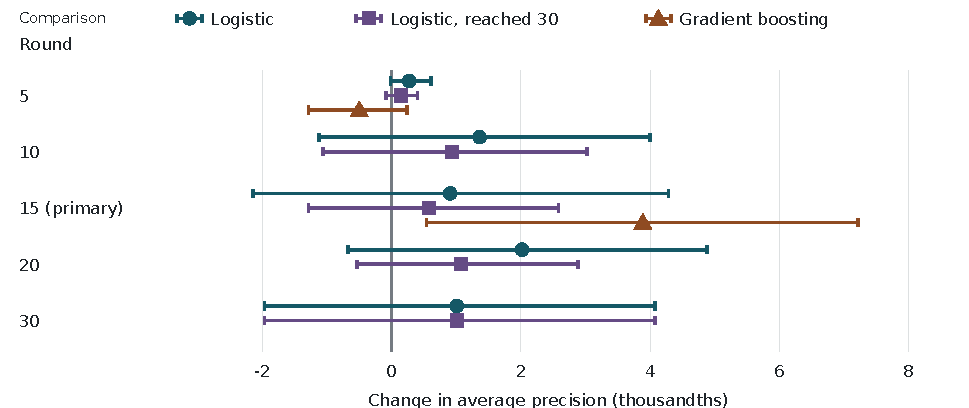
\includegraphics[width=\linewidth]{Fig1.pdf}
\captionof*{figure}{Figure 1. Change in average precision after adding four test proxies. Intervals are paired 95\% repository-bootstrap percentiles. The primary comparison is the logistic model at 15 rounds in the checkpoint-reaching population. The fixed cohort reaches 30 rounds at every comparison. Gradient boosting was evaluated at rounds 5 and 15.}
\end{minipage}\par
Restricting to the same reached-30 cohort yields K15 $\Delta$AP 0.000582591 with interval [-0.001289762, 0.002582330]. None of the fixed-population logistic M2 intervals excludes zero. This sensitivity analysis reduces changes in cohort membership across K, but does not equalize the information accumulated over time or remove unmeasured difficulty.

The nonlinear baseline gives a different secondary result (Table 5). At K15 its M0 AP is 0.660063 and M2 AP is 0.663951, with $\Delta$AP 0.003888397 and interval [0.000538769, 0.007222448]. At K5 the nonlinear contrast is negative and its interval includes zero. The K15 nonlinear finding is compatible with model-class-dependent predictive information in these proxies. It does not convert the primary logistic result into a positive finding, establish practical usefulness, or validate the proxy as true execution.

\begingroup\footnotesize\setlength{\tabcolsep}{3pt}
\begin{longtable}{>{\raggedright\arraybackslash}p{0.0572\textwidth}>{\raggedright\arraybackslash}p{0.0968\textwidth}>{\raggedright\arraybackslash}p{0.1672\textwidth}>{\raggedright\arraybackslash}p{0.1936\textwidth}>{\raggedright\arraybackslash}p{0.3652\textwidth}}
\caption*{Table 5. Prespecified secondary nonlinear baseline. The K15 M2 contrast is positive, but does not replace the primary logistic endpoint.}\\
\toprule
K & Model & AP & $\Delta$AP vs M0 & 95\% paired interval \\
\midrule
\endfirsthead
\toprule
K & Model & AP & $\Delta$AP vs M0 & 95\% paired interval \\
\midrule
\endhead
5 & M0 & 0.651683 & -- & -- \\
5 & M2 & 0.651181 & -0.000502 & [-0.001289, 0.000237] \\
15 & M0 & 0.660063 & -- & -- \\
15 & M2 & 0.663951 & 0.003888 & [0.000539, 0.007222] \\
\bottomrule
\end{longtable}
\endgroup
\subsection{6.4 Within-issue support, associations and stability}
The eligible pool contains 17,086 issues, of which 7,018 have outcome variation and contribute 69,453 rows to the issue-conditional analysis. There are 61,216 issue/configuration cells; 8,714 are outcome-discordant and contribute 25,028 rows, exceeding the support threshold for Model C. Groups contain at most 12 trajectories per issue and three per issue/configuration cell.

Table 6 and Figure 2 summarize the command-presence coefficient. At K10 its failure odds ratio is 0.8654 in ordinary logistic regression, 1.0804 conditional on issue, and 1.2510 conditional on issue/configuration. At K15 the corresponding values are 0.9545, 0.8921 and 0.8255. Every displayed interval spans one. The point estimates vary with adjustment and checkpoint; they do not support a single stable direction for a testing effect. The conditional populations also differ from the ordinary-regression population, so changes in odds ratios are not a pure decomposition of confounding.

\begingroup\footnotesize\setlength{\tabcolsep}{3pt}
\begin{longtable}{>{\raggedright\arraybackslash}p{0.0484\textwidth}>{\raggedright\arraybackslash}p{0.0660\textwidth}>{\raggedright\arraybackslash}p{0.1232\textwidth}>{\raggedright\arraybackslash}p{0.1232\textwidth}>{\raggedright\arraybackslash}p{0.1320\textwidth}>{\raggedright\arraybackslash}p{0.2332\textwidth}>{\raggedright\arraybackslash}p{0.1540\textwidth}}
\caption*{Table 6. Main command-presence associations with failure. A: ordinary logistic; B: issue conditional; C: issue/configuration conditional. Intervals use successful refits only; coverage is not established when refit failure is substantial.}\\
\toprule
K & Model & Rows & Groups & Failure OR & 95\% interval & Valid refits \\
\midrule
\endfirsthead
\toprule
K & Model & Rows & Groups & Failure OR & 95\% interval & Valid refits \\
\midrule
\endhead
10 & A & 159,867 & -- & 0.8654 & [0.7178, 1.0197] & 472/500 \\
10 & B & 69,453 & 7,018 & 1.0804 & [0.8449, 1.3730] & 500/500 \\
10 & C & 25,028 & 8,714 & 1.2510 & [0.8882, 1.8370] & 500/500 \\
15 & A & 159,867 & -- & 0.9545 & [0.8590, 1.0519] & 500/500 \\
15 & B & 69,453 & 7,018 & 0.8921 & [0.7750, 1.0532] & 497/500 \\
15 & C & 25,028 & 8,714 & 0.8255 & [0.6672, 1.0702] & 325/500 \\
\bottomrule
\end{longtable}
\endgroup
\par\noindent\begin{minipage}{\linewidth}
\centering
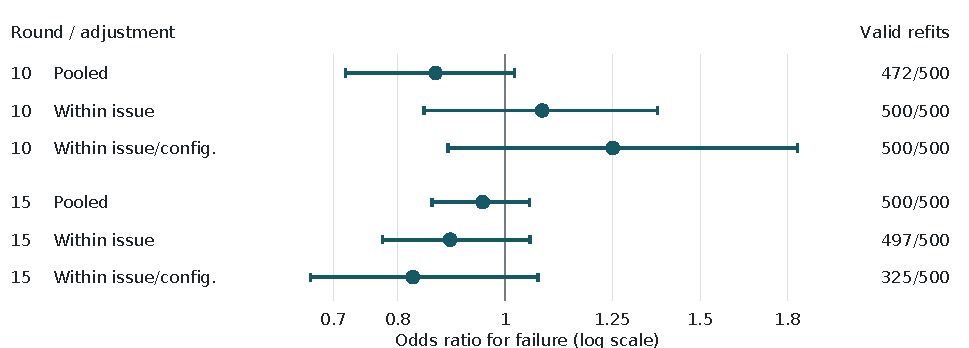
\includegraphics[width=\linewidth]{Fig2.pdf}
\captionof*{figure}{Figure 2. Association between detected command presence and task failure. The pooled and two conditional models adjust for the covariates in Section 5.3. Bars give 95\% percentiles among successful repository-bootstrap refits. Only 325 of 500 refits contributed to the round-15 interval within issue/configuration.}
\end{minipage}\par
All 14 point-estimate optimizations met the frozen acceptance criterion, but this does not certify a finite, well-identified maximum-likelihood estimate. Of the requested 7,000 refits, 860 failed convergence or rank checks. Main-model valid counts at K10 are 472/500, 500/500 and 500/500 for A/B/C; at K15 they are 500/500, 497/500 and 325/500. Configuration-specific valid counts range from 265/500 to 500/500. Sparse behavior and group support are important context, but the failure log does not distinguish every failure's causal source. We therefore report the counts rather than attributing all failures to one mechanism. The K10 SWE-agent/Qwen subgroup also has numerically extreme coefficients despite passing the gradient criterion; its magnitude and percentile intervals are not reliable effect estimates. Appendix D gives these diagnostics, all stability counts and configuration-specific command-presence outputs.

\section{7. Discussion}
The most direct result is the separation between a command signal and a verified behavior. The audit's high definite-command share can coexist with a substantially smaller execution-confirmed share, even before considering that the reconciled labels are AI-assisted and not an independent reference standard. Replacing unknown command evidence with a negative label would obscure precisely the cases where the trace cannot answer the measurement question. A useful measurement pipeline should preserve these distinctions rather than interpreting every detected runner invocation as a completed test run.

The primary prediction result is also more limited than a positive point estimate suggests. The broad proxy set improves AP by about nine ten-thousandths in the selected logistic comparison, with a cluster interval spanning both deterioration and improvement. This does not establish a practically useful early-warning feature. The positive K15 nonlinear secondary result deserves to be reported rather than suppressed: a richer functional form may extract information that the specified logistic model does not. However, model dependence, multiple exploratory contrasts and reuse of the historical snapshot make an independent frozen-dataset evaluation necessary before drawing a general claim. No decision threshold, human-review workload, runtime saving or downstream intervention benefit was tested here.

Within-issue adjustment answers a different question from held-out ranking. It compares trajectories sharing an issue, or an issue/configuration cell, rather than asking whether a score ranks unseen repositories well. The command-presence intervals span one in the main models and point directions change with the comparison. Even a more precise observational association would not settle causality. Testing can follow successful localization or respond to an already failing attempt, and the trace does not randomize these decisions.

Finally, computation completing is not the same as every interval being reliable. Repository resampling exposes weaknesses that can be hidden by reporting only point estimates. Some subgroup analyses retain little more than half of their requested bootstrap refits. Percentiles from those selected successful fits may not represent the intended resampling distribution. The failure counts are part of the result, not implementation details to discard. A future study should independently validate annotations, predefine how to handle weakly identified features, and evaluate any resulting rule on a genuinely new snapshot. Those are follow-up studies, not changes made to improve the present results after observing them.

\section{8. Limitations and research integrity}
\textbf{Measurement and shared assistance.} The review packages began as AI drafts and AI candidates resolved disagreements. Shared rule or model errors may survive review and create apparently high agreement. Owner attestations establish the declared provenance used by the project, not independent identity or chronology verification. The final labels must not be presented as independently human-adjudicated ground truth. No retrospective formal measurement interval corrects this limitation.

\textbf{Snapshot and outcome selection.} Only four historical configuration groups are represented, and 46,758 trajectories lack the modeled binary outcome. The analysis cannot establish behavior or predictive performance for those unknown-outcome trajectories, new models, new scaffolds, later dataset revisions or production settings. Repository separation reduces one form of leakage but does not prove that related projects, duplicated text or shared upstream code are absent across partitions.

\textbf{Prefix and task-selection effects.} A completed interaction round is not a uniform quantity of work. Conditioning on reaching K changes the sampled population, while the fixed reached-30 sensitivity still conditions on eventual duration. Short prefixes in the explanatory analyses differ from the checkpoint-reaching predictive populations. These choices limit temporal and causal interpretation even though they were fixed in advance.

\textbf{Inference and model dependence.} Test-bootstrap intervals condition on saved fitted predictors. Within-issue intervals exclude failed refits, sometimes at substantial rates. A small gradient can also coexist with numerically saturated coefficients: the implementation does not provide a formal separation diagnosis or establish a finite maximum-likelihood estimate for every subgroup. Multiple endpoints are exploratory and lack familywise correction; there is no equivalence margin, prospective power guarantee, or intervention experiment. A positive secondary interval cannot compensate for the primary interval spanning zero. Conversely, that primary result does not rule out every nonlinear or richer representation.



\section{9. Conclusion}
On this pinned coding-agent snapshot, detected test-command evidence and confirmed execution are distinct measurement targets. Adding four frozen command-related proxies does not establish incremental average precision in the preselected K15 logistic comparison. A positive nonlinear secondary contrast shows that the predictive conclusion depends on model class, while the main within-issue command-presence intervals span one and several bootstrap analyses are unstable. The evidence supports a qualified exploratory characterization of observable traces, not an independently validated behavioral gold standard, a causal claim about testing, or a demonstrated operational benefit.

\section{Statements and Declarations}
\textbf{Funding.} This research received no specific funding.

\textbf{Competing interests.} The authors declare that they have no competing interests.

\textbf{Data and code availability.} The raw trajectories are available from the pinned Open-SWE-Traces revision (NVIDIA 2026). The \href{https://github.com/fightforbelief/coding-agent-uncertainty-audit}{companion repository} provides the parser, analysis code, frozen protocol, and aggregate result tables. Weighted totals are available for the command and execution judgments in the 15-round detector-positive audit frame under each review version. A verification script recalculates the reported shares and checks the primary contrast and bootstrap refit counts against the archived tables. The research workspace retains the row-level audit judgments, exclusion IDs, feature matrix, held-out predictions and full refit records. The primary interval was independently recomputed from the stored scores using the same 1,000 paired repository draws.

\section{References}
Badertdinov I, Golubev A (2026) Interpreting coding agents through their behavioral trajectories. Workshop on Interpreting Agent Behavior, NeurIPS. \url{https://arxiv.org/abs/2611.17440}

Bouzenia I, Pradel M (2025) Understanding software engineering agents: a study of thought-action-result trajectories. ASE, pp 2846--2857. \url{https://doi.org/10.1109/ASE63991.2025.00234}

Cameron AC, Miller DL (2015) A practitioner's guide to cluster-robust inference. J Hum Resour 50:317--372. \url{https://doi.org/10.3368/jhr.50.2.317}

Jacobs AZ, Wallach H (2021) Measurement and fairness. FAccT, pp 375--385. \url{https://doi.org/10.1145/3442188.3445901}

Jimenez CE, Yang J, Wettig A, Yao S, Pei K, Press O, Narasimhan K (2024) SWE-bench: can language models resolve real-world GitHub issues? ICLR. \url{https://arxiv.org/abs/2310.06770}

NVIDIA (2026) Open-SWE-Traces, historical dataset snapshot. \href{https://huggingface.co/datasets/nvidia/Open-SWE-Traces/tree/c144d9d160dcd9f5ebcd9520d2d54111dda8b681}{Pinned dataset files}.

Scikit-learn developers (2026) Average precision score. \href{https://scikit-learn.org/stable/modules/generated/sklearn.metrics.average_precision_score.html}{API documentation}.

Statsmodels developers (2026) ConditionalLogit, release 0.14.6. \href{https://www.statsmodels.org/v0.14.6/generated/statsmodels.discrete.conditional_models.ConditionalLogit.html}{API documentation}.

Wang X, Li B, Song Y et al (2025) OpenHands: an open platform for AI software developers as generalist agents. ICLR. \url{https://arxiv.org/abs/2407.16741}

Wang Y, Pradel M, Liu Z (2026) Are solved issues in SWE-bench really solved correctly? An empirical study. ICSE. \url{https://doi.org/10.1145/3744916.3764576}

Yang J, Jimenez CE, Wettig A, Lieret K, Yao S, Narasimhan K, Press O (2024) SWE-agent: agent-computer interfaces enable automated software engineering. NeurIPS. \url{https://arxiv.org/abs/2405.15793}

\section{Appendix A. Relationship to the historical analysis}
The original frozen K5 analysis scored 20,118 test trajectories and compared a historical structural model with that model plus the original strict explicit-test-failure signal. Structural AP was 0.640960128243 and augmented AP was 0.641026019969, giving $\Delta$AP 0.000065891727 and a paired repository-bootstrap interval [0.000005607830, 0.000132822866]. The OpenHands-only historical replication also matched its stored predictions and metrics. The historical report is archived separately in the repository.

The current extension excludes all audit identifiers, expands the proxy set, uses a separate command detector, adds checkpoints and selects K15 as its primary exploratory endpoint. Even its K5 M1 cell is therefore not identical to the historical specification. The old result and the new results are not two independent studies; they reuse the snapshot. We do not interpret their numerical differences as an intervention effect, a correction of the historical result, or a before/after improvement.

\section{Appendix B. Audit frames and proxy support}
The frozen primary strata use parser-eligible trajectories and the following rule outputs: A requires high-confidence R5 command presence; B requires high-confidence R15 presence, R5 detector absence, and no missing R5 execution command; C requires R15 detector absence and no missing R15 execution command; D requires R15 detector absence with a missing R15 execution command. The additional AMB5/AMB15 frames require the corresponding ambiguous-command flag. The reported R15 positive summary combines A and B; it is not a blanket estimate for all possible R15-positive histories, including those outside these eligibility rules. Each configuration's $N_h/n_h$ is retained in the sampling design.

The command-status categories are definite test command, definite no-test command, ambiguous, command unrecoverable and insufficient evidence. Separate fields retain execution confirmation, process status, pre-test failure detail, output status and mixed pass/failure composition. An explicit failure and a process-started status are not equivalent to successful test execution. Neither same-runner failure-then-pass nor an explicit passing summary establishes that the final patch resolves its issue.

\begingroup\footnotesize\setlength{\tabcolsep}{3pt}
\begin{longtable}{>{\raggedright\arraybackslash}p{0.0528\textwidth}>{\raggedright\arraybackslash}p{0.1672\textwidth}>{\raggedright\arraybackslash}p{0.2200\textwidth}>{\raggedright\arraybackslash}p{0.2024\textwidth}>{\raggedright\arraybackslash}p{0.2376\textwidth}}
\caption*{Table A1. Support for frozen detector proxies among checkpoint-reaching eligible trajectories across all prediction partitions.}\\
\toprule
K & Eligible n & Command present & Explicit failure & Failure-then-pass \\
\midrule
\endfirsthead
\toprule
K & Eligible n & Command present & Explicit failure & Failure-then-pass \\
\midrule
\endhead
5 & 159,867 & 1,020 & 64 & 1 \\
10 & 159,864 & 14,142 & 1,303 & 124 \\
15 & 159,823 & 35,816 & 4,659 & 715 \\
20 & 159,543 & 56,764 & 10,117 & 2,271 \\
30 & 156,326 & 86,639 & 23,547 & 8,982 \\
\bottomrule
\end{longtable}
\endgroup
Table A1 counts detector outputs among checkpoint-reaching known-label, non-audit trajectories pooled across the three prediction partitions. These are descriptive support counts, not additional predictive evaluations. The explanatory models at K10/K15 retain shorter trajectories as described in Section 5.3, so their denominators differ. The companion tables include configuration-specific command-presence estimates and the retained within-issue coefficients.


\section{Appendix C. Additional predictive results}
\begingroup\footnotesize\setlength{\tabcolsep}{3pt}
\begin{longtable}{>{\raggedright\arraybackslash}p{0.0440\textwidth}>{\raggedright\arraybackslash}p{0.0704\textwidth}>{\raggedright\arraybackslash}p{0.1232\textwidth}>{\raggedright\arraybackslash}p{0.1232\textwidth}>{\raggedright\arraybackslash}p{0.1232\textwidth}>{\raggedright\arraybackslash}p{0.1232\textwidth}>{\raggedright\arraybackslash}p{0.2728\textwidth}}
\caption*{Table A2. Complete main-population logistic metrics. All AP contrasts use the same K-specific M0. Intervals are unadjusted exploratory paired-bootstrap summaries.}\\
\toprule
K & Model & AP & AUROC & Brier & $\Delta$AP & 95\% paired interval \\
\midrule
\endfirsthead
\toprule
K & Model & AP & AUROC & Brier & $\Delta$AP & 95\% paired interval \\
\midrule
\endhead
5 & M0 & 0.640799 & 0.557202 & 0.240135 & -- & -- \\
5 & M1 & 0.640868 & 0.557345 & 0.240117 & 0.000069 & [0.000003, 0.000169] \\
5 & M2 & 0.641071 & 0.557598 & 0.240090 & 0.000272 & [-0.000019, 0.000607] \\
10 & M0 & 0.639777 & 0.559388 & 0.240105 & -- & -- \\
10 & M1 & 0.640038 & 0.559556 & 0.240072 & 0.000261 & [-0.000304, 0.000849] \\
10 & M2 & 0.641138 & 0.560599 & 0.239970 & 0.001361 & [-0.001125, 0.003995] \\
15 & M0 & 0.641246 & 0.567562 & 0.239811 & -- & -- \\
15 & M1 & 0.641611 & 0.568702 & 0.239705 & 0.000365 & [-0.000606, 0.001310] \\
15 & M2 & 0.642153 & 0.569493 & 0.239553 & 0.000907 & [-0.002150, 0.004284] \\
20 & M0 & 0.646857 & 0.573203 & 0.239113 & -- & -- \\
20 & M1 & 0.647583 & 0.574814 & 0.238977 & 0.000726 & [-0.000423, 0.001895] \\
20 & M2 & 0.648875 & 0.576545 & 0.238673 & 0.002019 & [-0.000681, 0.004885] \\
30 & M0 & 0.661830 & 0.586637 & 0.236871 & -- & -- \\
30 & M1 & 0.662082 & 0.587018 & 0.236837 & 0.000252 & [-0.000072, 0.000600] \\
30 & M2 & 0.662838 & 0.588424 & 0.236574 & 0.001008 & [-0.001968, 0.004082] \\
\bottomrule
\end{longtable}
\endgroup
Table A2 contains all main-population logistic metrics. M1 and M2 intervals compare each model with the same K-specific M0. All prediction contrasts have 1,000 valid paired bootstrap draws. Model-selection grids, selected C values and M2 standardized coefficients are preserved in the cell-level result files. No failed prediction-bootstrap draws occurred.

\begingroup\footnotesize\setlength{\tabcolsep}{3pt}
\begin{longtable}{>{\raggedright\arraybackslash}p{0.0528\textwidth}>{\raggedright\arraybackslash}p{0.1408\textwidth}>{\raggedright\arraybackslash}p{0.1760\textwidth}>{\raggedright\arraybackslash}p{0.1760\textwidth}>{\raggedright\arraybackslash}p{0.3344\textwidth}}
\caption*{Table A3. Fixed reached-30 population, M2 versus M0 at each checkpoint.}\\
\toprule
K & Test n & M2 AP & $\Delta$AP & 95\% paired interval \\
\midrule
\endfirsthead
\toprule
K & Test n & M2 AP & $\Delta$AP & 95\% paired interval \\
\midrule
\endhead
5 & 19,614 & 0.644254 & 0.000139 & [-0.000088, 0.000402] \\
10 & 19,614 & 0.644045 & 0.000934 & [-0.001059, 0.003027] \\
15 & 19,614 & 0.645746 & 0.000583 & [-0.001290, 0.002582] \\
20 & 19,614 & 0.651458 & 0.001079 & [-0.000533, 0.002885] \\
30 & 19,614 & 0.662838 & 0.001008 & [-0.001968, 0.004082] \\
\bottomrule
\end{longtable}
\endgroup
Table A3 reports the M2 sensitivity contrast on the fixed reached-30 population. Its test cohort has 19,614 trajectories at every checkpoint. The fixed training and validation cohorts have 110,791 and 25,921 trajectories, respectively. The companion tables give the complete checkpoint metrics.


\section{Appendix D. Within-issue stability and configuration comparisons}
\begingroup\footnotesize\setlength{\tabcolsep}{3pt}
\begin{longtable}{>{\raggedright\arraybackslash}p{0.2200\textwidth}>{\raggedright\arraybackslash}p{0.0616\textwidth}>{\raggedright\arraybackslash}p{0.2200\textwidth}>{\raggedright\arraybackslash}p{0.1892\textwidth}>{\raggedright\arraybackslash}p{0.1892\textwidth}}
\caption*{Table A4. Complete bootstrap refit accounting (500 requested per analysis). A completed point estimate does not imply all resamples were estimable.}\\
\toprule
Analysis & K & Point-estimate rows & Valid refits & Failed refits \\
\midrule
\endfirsthead
\toprule
Analysis & K & Point-estimate rows & Valid refits & Failed refits \\
\midrule
\endhead
A & 10 & 159,867 & 472 & 28 \\
B & 10 & 69,453 & 500 & 0 \\
B: OH/M & 10 & 4,769 & 307 & 193 \\
B: OH/Q & 10 & 7,348 & 500 & 0 \\
B: SWE/M & 10 & 7,041 & 500 & 0 \\
B: SWE/Q & 10 & 5,870 & 265 & 235 \\
C & 10 & 25,028 & 500 & 0 \\
A & 15 & 159,867 & 500 & 0 \\
B & 15 & 69,453 & 497 & 3 \\
B: OH/M & 15 & 4,769 & 330 & 170 \\
B: OH/Q & 15 & 7,348 & 500 & 0 \\
B: SWE/M & 15 & 7,041 & 500 & 0 \\
B: SWE/Q & 15 & 5,870 & 444 & 56 \\
C & 15 & 25,028 & 325 & 175 \\
\bottomrule
\end{longtable}
\endgroup
Refits failed the rank or convergence checks. Conditioning on successful fits makes nominal coverage uncertain, particularly in the K10 SWE/Q subgroup.

\begingroup\footnotesize\setlength{\tabcolsep}{3pt}
\begin{longtable}{>{\raggedright\arraybackslash}p{0.2200\textwidth}>{\raggedright\arraybackslash}p{0.0528\textwidth}>{\raggedright\arraybackslash}p{0.1584\textwidth}>{\raggedright\arraybackslash}p{0.2816\textwidth}>{\raggedright\arraybackslash}p{0.1672\textwidth}}
\caption*{Table A5. Configuration-specific issue-conditional command-presence odds ratios for task failure. Intervals use successful refits only.}\\
\toprule
Configuration & K & Failure OR & 95\% interval & Valid refits \\
\midrule
\endfirsthead
\toprule
Configuration & K & Failure OR & 95\% interval & Valid refits \\
\midrule
\endhead
B: OH/M & 10 & 1.6313 & [0.5906, 3.5788] & 307/500 \\
B: OH/Q & 10 & 2.0337 & [0.2445, 36.8278] & 500/500 \\
B: SWE/M & 10 & 1.1663 & [0.7137, 1.7511] & 500/500 \\
B: SWE/Q & 10 & 2.83e-15 & [1.55e-15, 4.87e-15] & 265/500 \\
B: OH/M & 15 & 0.8380 & [0.5146, 1.3270] & 330/500 \\
B: OH/Q & 15 & 1.1968 & [0.6710, 2.3868] & 500/500 \\
B: SWE/M & 15 & 0.7920 & [0.5615, 1.1225] & 500/500 \\
B: SWE/Q & 15 & 0.6887 & [0.2048, 2.8978] & 444/500 \\
\bottomrule
\end{longtable}
\endgroup
OH and SWE denote OpenHands and SWE-agent. M and Q denote MiniMax and Qwen. Each model conditions on outcome-discordant issues within one configuration.

The K10 SWE/Q coefficients show numerical saturation. The command-presence odds ratio was $2.83\times10^{-15}$, compared with $1.33\times10^{21}$ for command count and $4.75\times10^{55}$ for explicit failure. The last estimate had identical bootstrap percentiles. A small gradient and a matching reference likelihood do not guarantee a finite maximum-likelihood estimate. These magnitudes have no reliable behavioral interpretation.
\end{document}
